\documentclass[11pt,reqno]{article}
 
\usepackage[margin=0.7in]{geometry} 
\usepackage{graphicx}
\usepackage{amsmath,amsthm,amssymb}
\usepackage{easylist}
\usepackage{enumerate}
\usepackage{cases}

\usepackage{listings}
\usepackage{color}

\usepackage{changepage}

\definecolor{dkgreen}{rgb}{0,0.6,0}
\definecolor{gray}{rgb}{0.5,0.5,0.5}
\definecolor{mauve}{rgb}{0.58,0,0.82}

\lstset{frame=tb,
  language=matlab,
  aboveskip=3mm,
  belowskip=3mm,
  showstringspaces=false,
  columns=flexible,
  basicstyle={\small\ttfamily},
  numbers=none,
  numberstyle=\tiny\color{gray},
  keywordstyle=\color{blue},
  commentstyle=\color{dkgreen},
  stringstyle=\color{mauve},
  breaklines=true,
  breakatwhitespace=true,
  tabsize=3,
  frame=single                    % adds a frame around the code
}
 
\newcommand{\N}{\mathbb{N}}
\newcommand{\R}{\mathbb{R}}
\newcommand{\Z}{\mathbb{Z}}
\newcommand{\ind}{\setlength{\parindent}{5ex} \indent}
\newcommand{\CI}{\mathrel{\perp\mspace{-10mu}\perp}}
\newcommand{\nCI}{\centernot{\CI}} % the symbol for conditional independent

\newenvironment{parind}{\begin{adjustwidth}{0.5cm}{}}{\end{adjustwidth}}
\begin{document}
\title{\textbf {Brief Description of the DP Algorithm Design}}
\date{}
\maketitle
% --------------------------------------------------------------
%                         Start here
% --------------------------------------------------------------
\subsection*{Objective} 
\paragraph{} To estimate the maximum expected profit in $T$ days given the current storage condition.
\subsection*{Mathematical Model}
\paragraph{} The entire storage can be divide into $m$ categories and the items belonging to the $i$th category are expiring in $i$ days where $i \in [0,m-i]$. Note the maximum number of items within each category is limited to $k$. We store the number of items in all the categories in a $m$ dimensional vector where the first element represents the number of items to be expired today and the last element represents the number of items to be expired in $m - 1$ days. We denote the vector as $X$ and $X_{t}$ is the storage status of the $t$-th day.
\paragraph{} Everyday in the evening, the shop manager has to clean up the items that has been expired on that day and each item has a disposal cost $\theta$. Next he shall decide the depletion amount. For each item depleted, an amount of salvage denoted as $s$ will be recovered and counted into benefits. And after the depletion, all the items remained in the storage will be charged a holding cost each which is denoted as $h$. And in the morning of the following day, the manager will decide the total amount of items to order, the order cost is $c$ per item. During the opening hours, those items which are going to be expired will be sold based on the possion distribution, and the selling price is $r$. Therefore the net income for the entire period can be expressed as 
\begin{eqnarray*}
Profit = &+&numDeplete \cdot s \\
&-& totalNum \cdot h \\
&-& numOrder \cdot c \\
&+& min(\textbf{D},~ totalNum + numOrder) \cdot r \\
&-& X_{0} \cdot \theta
\end{eqnarray*}
where 
\begin{itemize}
        \item $numDeplete$ is the number of items been depleted on the night before 
        \item $totalNum$ is the number of items remained in the storage after depletion but before the next ordering
        \item $D$ is the random variable to denote the number of items sold in a day. And it follows the Possion distribution.
\end{itemize}

\paragraph{} So in order to find out the maximum expected value, we have the following recursion relation:
$$V_{t}(X_{t}) = max_{z \in Z, q \in Q}(\textbf{E}[Profit(X_{t}, z, q, \textbf{D})] +  \alpha \textbf{E}[V_{t+1}(S(X_{t}, z, q), z, q, \textbf{D})]) $$
where 
\begin{itemize}
        \item $z$ represents the number of depletion with range $Z$, and $q$ is the number of ordering with the limit $Q$
        \item $S$ is the function to evaluate $X_{t + 1}$ given $X_{t}$, $z, q$
\end{itemize}

\paragraph{} Therefore $V_{t}$ is attainable once given $V_{t + 1}$.
\paragraph{} We shall start from the table $V_{T}$, in which all the entries equal to zero, to recursively update the table $V_{i}$~($i = T-1, T-2, \dots)$ and go all the way down to $i = 0$, which is the table of today.

\subsection*{Approaches}
\paragraph{} The problem itself has some fine features leading to a simpler solution. 

        \begin{itemize}
                % add more details and properties of the tree here
                \item \textbf{Inherited Relation of Depletion }\hfill \\ All the state values within the table shall be organized in a tree, where the  optimal depletion number of a child node has some relation with its parent node. \\
                        For example, for a problem with $ m = 3, ~ k = 2$, the following structure can be obtained.
                        \begin{figure}[ht]
                                \centering
                                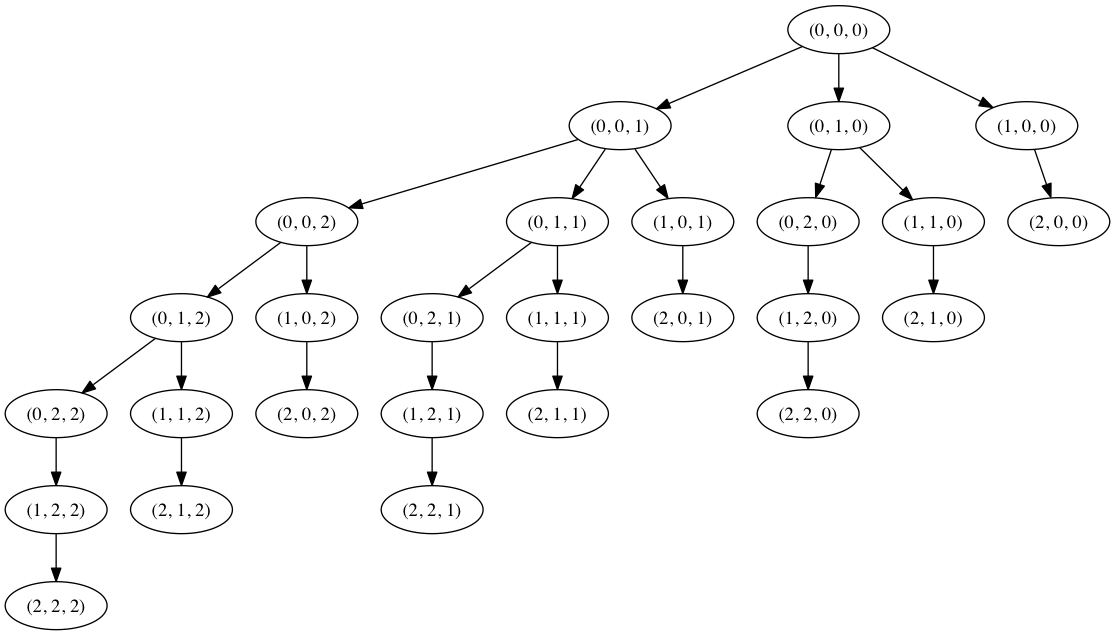
\includegraphics[width = 160mm]{treeStruct.png}
                                \caption{ The tree structure for $m = 3$, $k = 2$}
                        \end{figure}
                \item \textbf{Limited Demands per day }\hfill \\ There is a upper limit for the number of customers that may visit the shop everyday. And maximum number should be rather small ( hopefully less than a hundred).  So instead of launching the kernels for thousands of times to get better estimation, we may simply calculate the result for every demand within the range and adjust the result by the weights given by the Possion distribution. 
        \end{itemize}
        
        \paragraph{} Based on the above analysis of the problem, a parallel process to deal with the problem can be described as follows. Take the problem discussed above as the example. 
        \begin{figure}[ht]
                \centering
                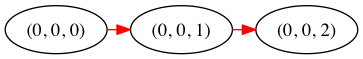
\includegraphics[width = 90mm]{traversal1.png}
                \caption{step 1}
        \end{figure}
        \begin{figure}[ht]
                \centering
                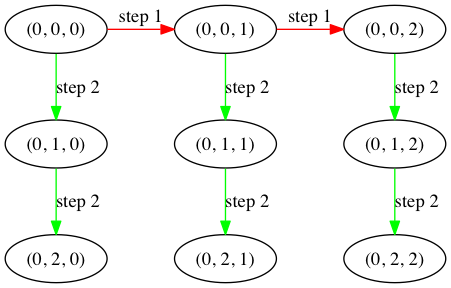
\includegraphics[width = 90mm]{traversal2.png}
                \caption{step 2}
        \end{figure}
        \begin{figure}[ht]
                \centering
                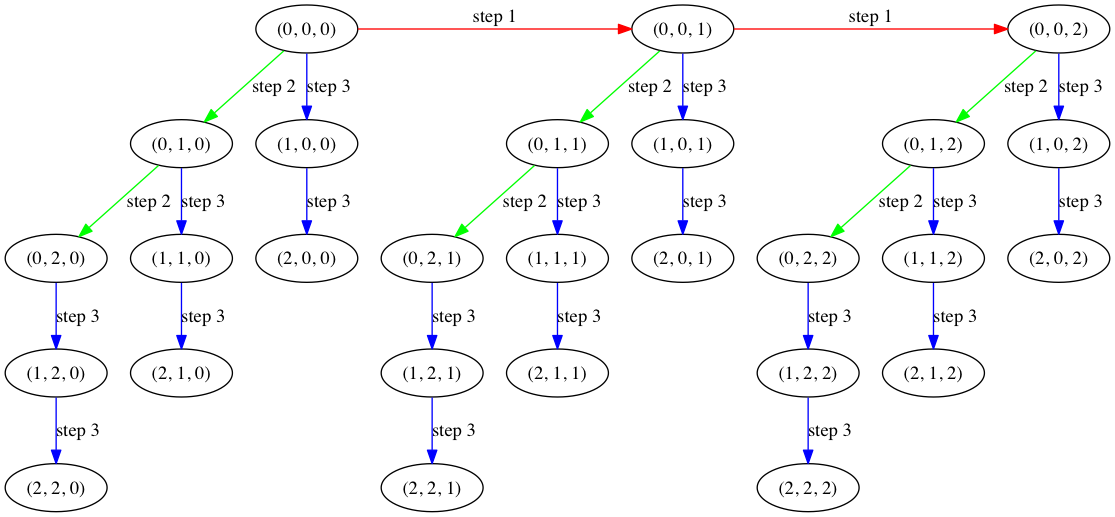
\includegraphics[width = 180mm]{traversal3.png}
                \caption{step 3}
        \end{figure}

        \paragraph{} So in total $m$ iterations are needed and within each iteration $k ^{i - 1}$ threads operate in parallel where $i$ is the index of the iteration.  
\subsection*{Algorithm Implementation}
\paragraph{} There are three tables kept in the GPU memory all the time, the $V_{t + 1}$, the $V_{t}$, and a table holding the all the depletion amount for each state of $V_{t + 1}$. And what we are going to do here is to update the table of $V_{t}$ based on $V_{t + 1}$ and the depletion information.
\paragraph{} As has been discussed above, the $V_{t}$ table will be updated in $m$ iterations and within each iteration, $k_{i - 1}$ threads will be in useo

\begin{figure}[c]
        \centering
        \includegraphics{<+file+>}
        \caption{<+caption text+>}
        \label{fig:<+label+>}
\end{figure}<++>

% --------------------------------------------------------------
% 			End of the file
% --------------------------------------------------------------
 
\end{document}
